\chapter{Systemidentifikation im Zeitbereich}

\section{Methode der kleinsten Fehlerquadrat}
Die Methode der Kleinste-Quadrate-Schätzung (LSQ) wird in diesem Kapitel vorgestellt.
Eine der Kernaufgaben vieler Ingenieure einen belastbaren Zusammenhang zwischen gemessenen Werten zu finden. Diese Zusammenhänge können  Näherungsweise durch folgendes lineares Modell beschrieben werden:  
\begin{equation}
    z = H\cdot x+v 
\end{equation}
mit 
\[z = [z_{1} \, z_{2} \, ...\,  z_{m} ]^T =\, m\times 1 \; \text{Messungsvektor} \]
\[ H= \; m\times n \;\text{bekannte Matrix } \]
\[ v = \;\text{unbekannter Rauschterm } \]
\[ x= \; n\times 1 \;\text{unbekannter Parametervektor } \]
 \noindent LSQ kann hilfreich werden, um zum Beispiel die Schätzung von Modellparametern bei Systemidentifikation durchzuführen.  
Gesucht ist ein Schätztwert $\hat{x}$ für Parametervektor. Der Restfehlervektor $e$ lautet:
\begin{equation}
    e = z - H\cdot \hat{x} \\
\end{equation}
Die Idee ist ein Wert von $\hat{x}$ zu finden, das die 2-Norm des Restfehlervektors minimieren soll. Das quadratische Zielfunktional $J$ ist gegeben durch: 
\begin{align}
   \begin{split}
     J = 1/2 \cdot e^{T} \cdot e \\
     = 1/2 \cdot {(z- H\hat{x})}^{T}\cdot(z- H\hat{x}) \\
     = 1/2 \cdot (z^{T} -{\hat{x}}^{T}H^{T})\cdot(z- H\hat{x}) \\
     = 1/2 \cdot z^{T}z - z^{T}H\hat{x} + 1/2\cdot {\hat{x}}^{T}A\hat{x}  \\
   \end{split}
\end{align}
mit $A = H^{T}H$. Die Lösung des Minimierungsproblems lautet dann:
\begin{equation}
    \hat{x}= {(H^{T} H)}^{-1} \cdot H^{T} z 
\end{equation}
\subsection{Bestimmung von Aerodynamischen Parametern anhand LSQ} 
Die Zustandsraumdarstellung \eqref{eq:laengsbewegung} liefert folgende Gleichungen: 
\[\Delta\dot \alpha-q =  \frac{Z_{\alpha}\Delta\alpha}{V_0} + \frac{Z_{\nu}\Delta V_{A}}{V_0} + \frac{Z_{\eta}\Delta\eta}{V_0} - \frac{X_{\delta F}\sin{(\alpha_0 + i_F)}\cdot\Delta\delta_F}{V_0}\] 
\[ \dot q = M_{\alpha}\Delta\alpha + M_{q}q + M_{\nu}\Delta V_A + M_{\eta}\Delta\eta + M{\delta F}\Delta\delta_F\]
\[\Delta\dot V_A = X_{\alpha}\Delta\alpha +  X_{\nu}\Delta V_A + X_{\eta}\Delta\eta + X_{\delta F}\cos{(\alpha_0 + i_F)}\cdot\Delta\delta_ \]
\[\Delta \dot \gamma = \frac{- Z_{\alpha}\Delta\alpha}{V_0} + \frac{- Z_{\nu}\Delta V_{A}}{V_0} + \frac{- Z_{\eta}\Delta\eta}{V_0} + \frac{X_{\delta F}\sin{(\alpha_0 + i_F)}\cdot\Delta\delta_F}{V_0}\]
Welche zu dem folgenden linearen Gleichungssystem umgeformt werden können: 
\begin{equation}
    z_{L}= H_{L}\cdot x + v
\end{equation}
Sodass:
\setcounter{MaxMatrixCols}{15}
\[z_{L} = (\Delta\dot \alpha-q \;\; \dot q \;\; \Delta\dot V_A)^T\] \\
\[ H_{L} = \begin{pmatrix}
0&0&0& \frac{-\sin{(\alpha_0 + i_F)}\cdot\Delta\delta_F}{V_0} & \frac{\Delta\alpha}{V_0}& \frac{\Delta V_A}{V_0} & \frac{\Delta\eta}{V_0} &0&0&0&0&0   \\
0&0&0&0&0&0&0 &\Delta\alpha & q & \Delta V_A & \Delta\eta & \Delta\delta_F \\
\Delta\alpha &  \Delta V_A & \Delta\eta & \cos{(\alpha_0 + i_F)}\cdot\Delta\delta_F &0&0&0&0&0&0&0&0 
\end{pmatrix}\] \\
\[x = (X_{\alpha}\; 
X_{\nu}\;
X_{\eta}\;
X_{\delta_F}\; 
Z_{\alpha}\; 
Z_{\nu}\;
Z_{\eta}\;
M_{\alpha}\;
M_{q}\;
M_{\nu}\;
M_{\eta}\;
M_{\delta_F}\;)^T
 \]
 \section{Ergebnisse}
 
 Anschließend werden die Ergebnisse in diesem Kapitel kurz vorgestellt.\par
 \noindent Nach der Schätzung der Einträge der Matrizen $A$ und $B$, wird das Anfangswertproblem \eqref{eq:laengsbewegung} auf das gesamte Zeitintervall gelöst. Bei allen Simulationen sind die Filterparamtern von Kapitel 3.4.2 gewählt.\par
 \noindent In Abbildung \ref{fig:Ergebnisse_zmlsq} wird die Lösung Anhand ein Matrix-LSQ-Verfahren dargestellt. Die Ergebnisse zeigen eine relativ präzise Approximation. Das verfahren ist sehr schnell und einfach zu implementieren in vergleich zur LSQ-Methode.  Allerdings steht es aus flugmechanischer Sicht Abweichungen in System- und Eingangsmatrix. Die Matrizen $A$ und $B$ lauten: 
 \[ A = \begin{pmatrix}
 -0.1940 & 0.005 & -0.0002 & -0.0540 \\
 -38.9899 & -12.8888 & 0.3632 & -4.2686 \\
 -6.1506 & -0.1501 & -0.0589 & -5.0107 \\
 0.4433 & 0.0427 & 0.0023 & 0.0818
 \end{pmatrix}
 \] 
 \[ B = \begin{pmatrix}
 -0.0267 & -0.0164 \\ 
 -26.1377 & -12.9651 \\
 -0.7414 & 4.6092 \\
 0.0477 & -0.1328
 \end{pmatrix}
 \]
 \noindent Die Abbildung \ref{fig:Ergebnisse_zlsq} stellt die Lösung Anhand das LSQ-Verfahren. Die Methode liefert keine sonderlich guten Ergebnisse. 
 \begin{figure}[h!]
	\centering
	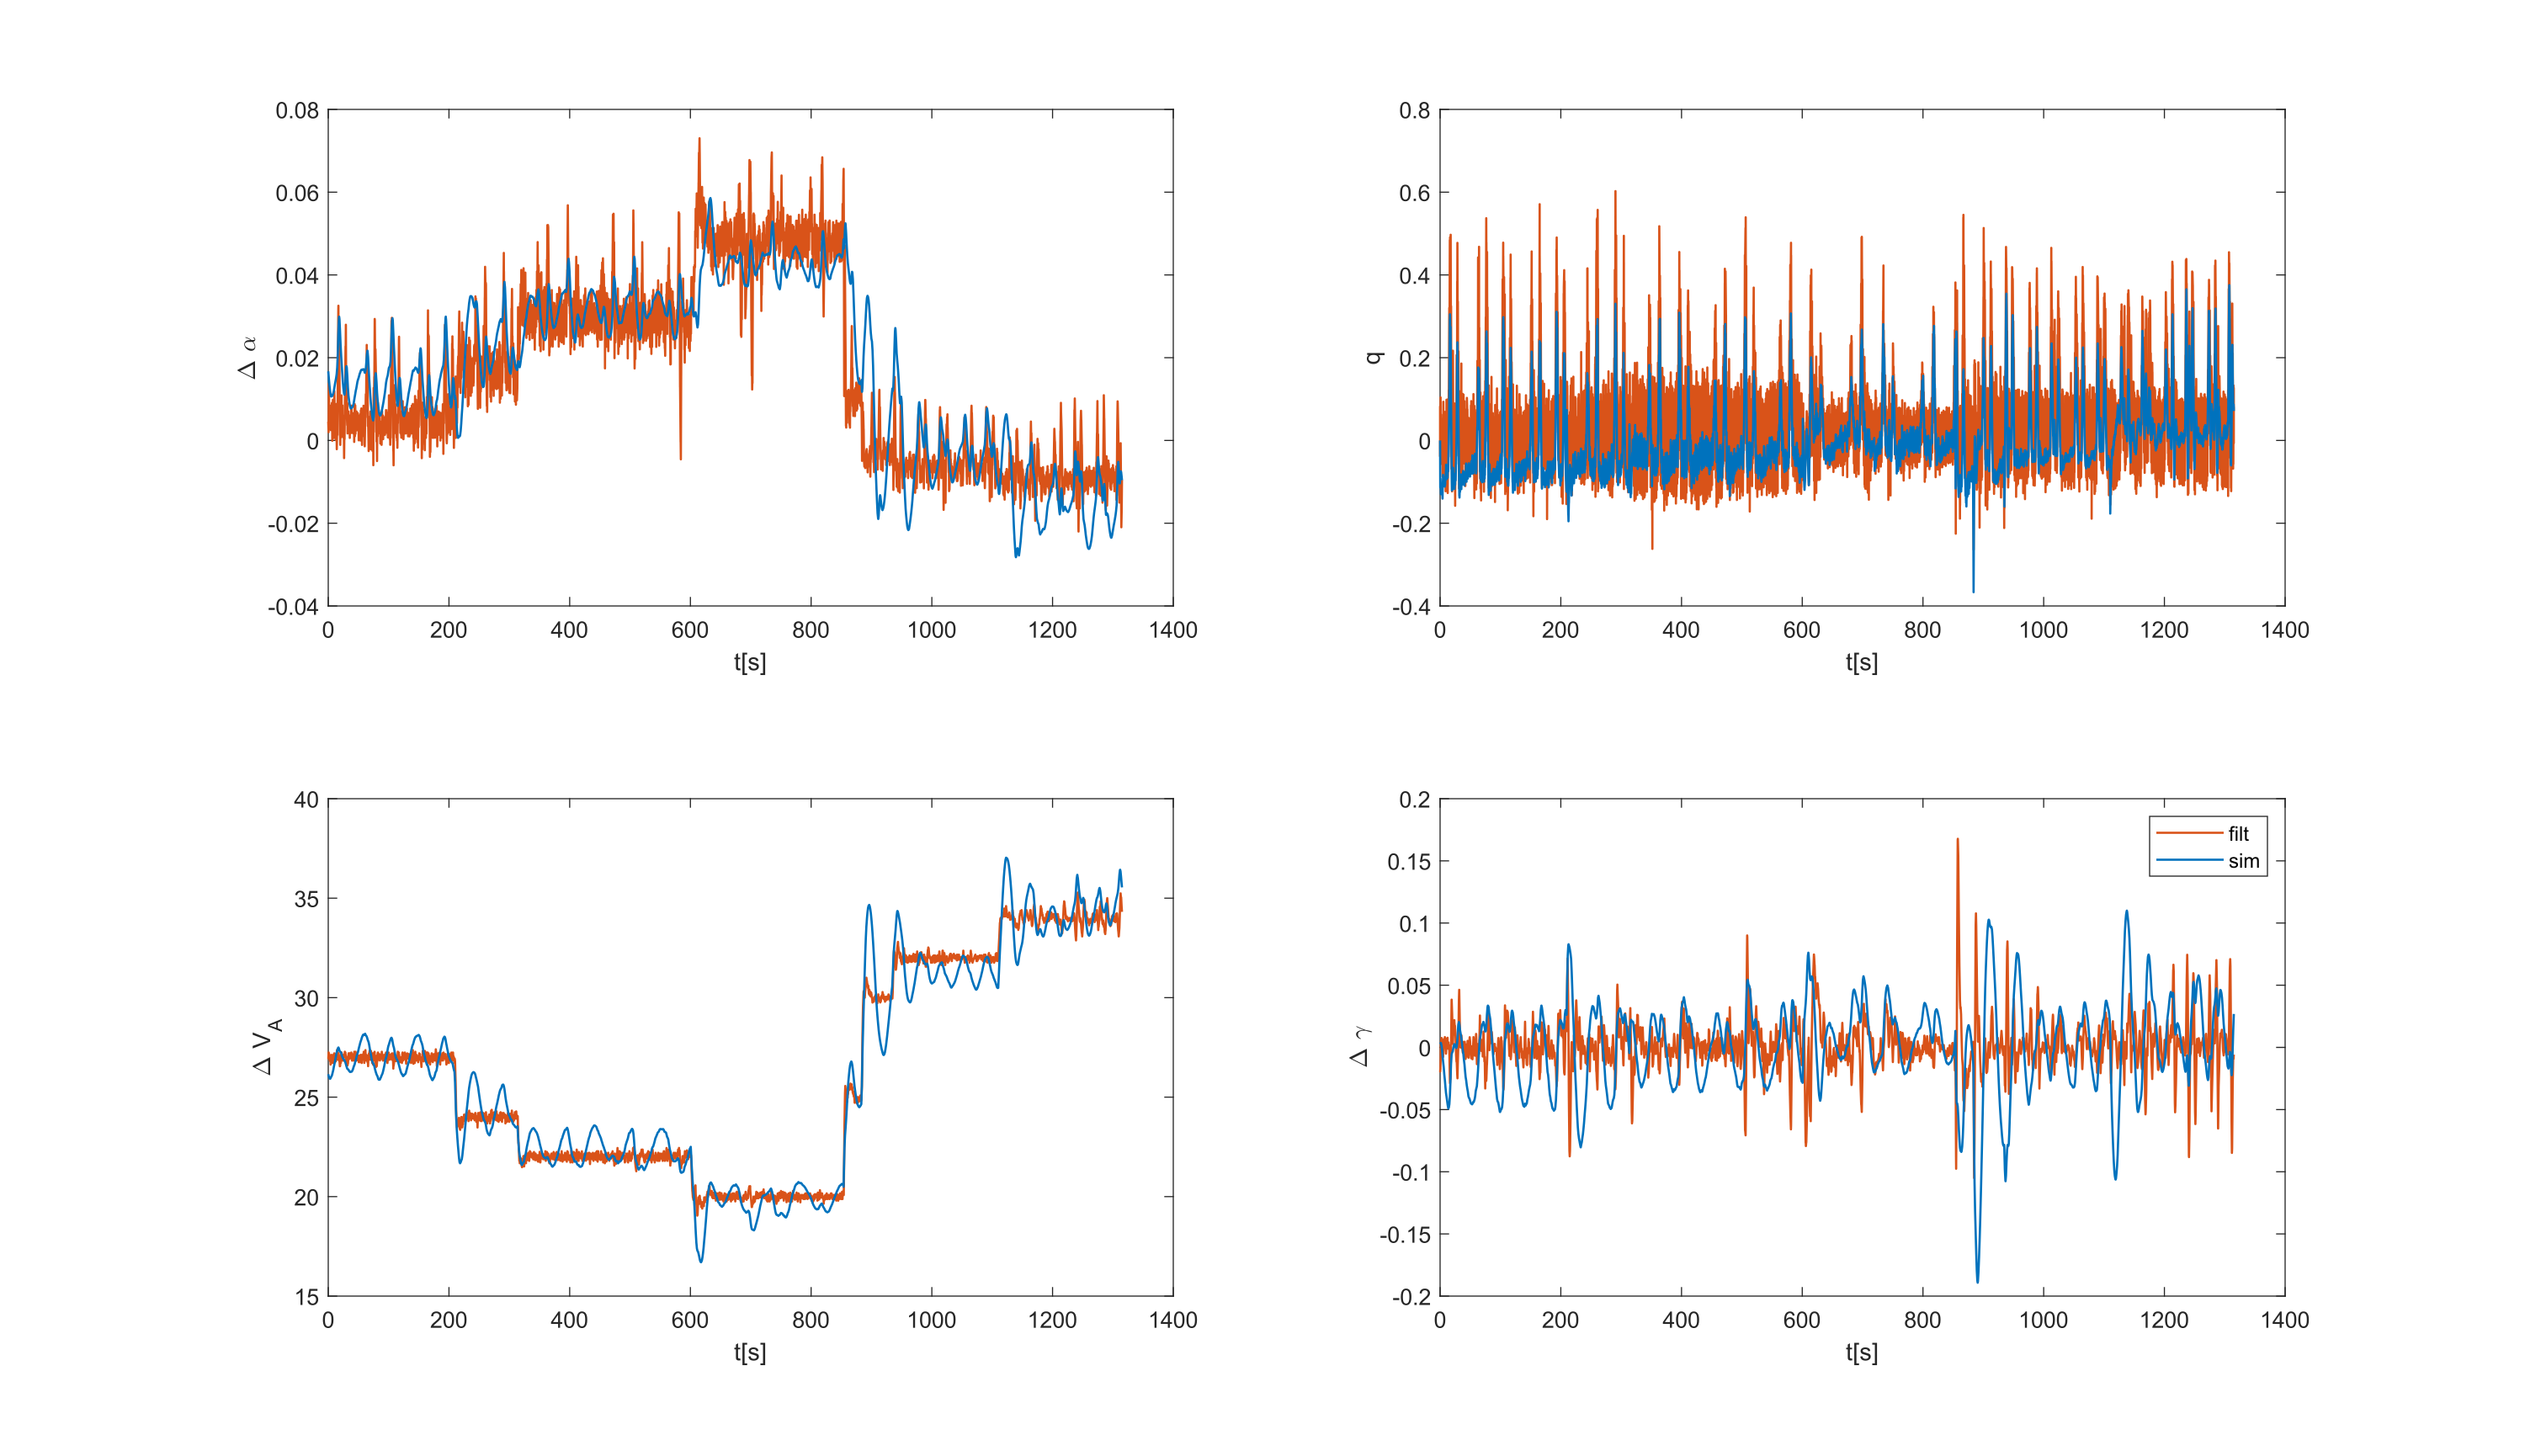
\includegraphics[trim=100 0 100 0,clip,width=1\linewidth]{LS.png}
	\caption{Ergebnisse Anhand Matrix-LSQ }
    \label{fig:Ergebnisse_zmlsq}
\end{figure}

 \begin{figure}[h!]
	\centering
	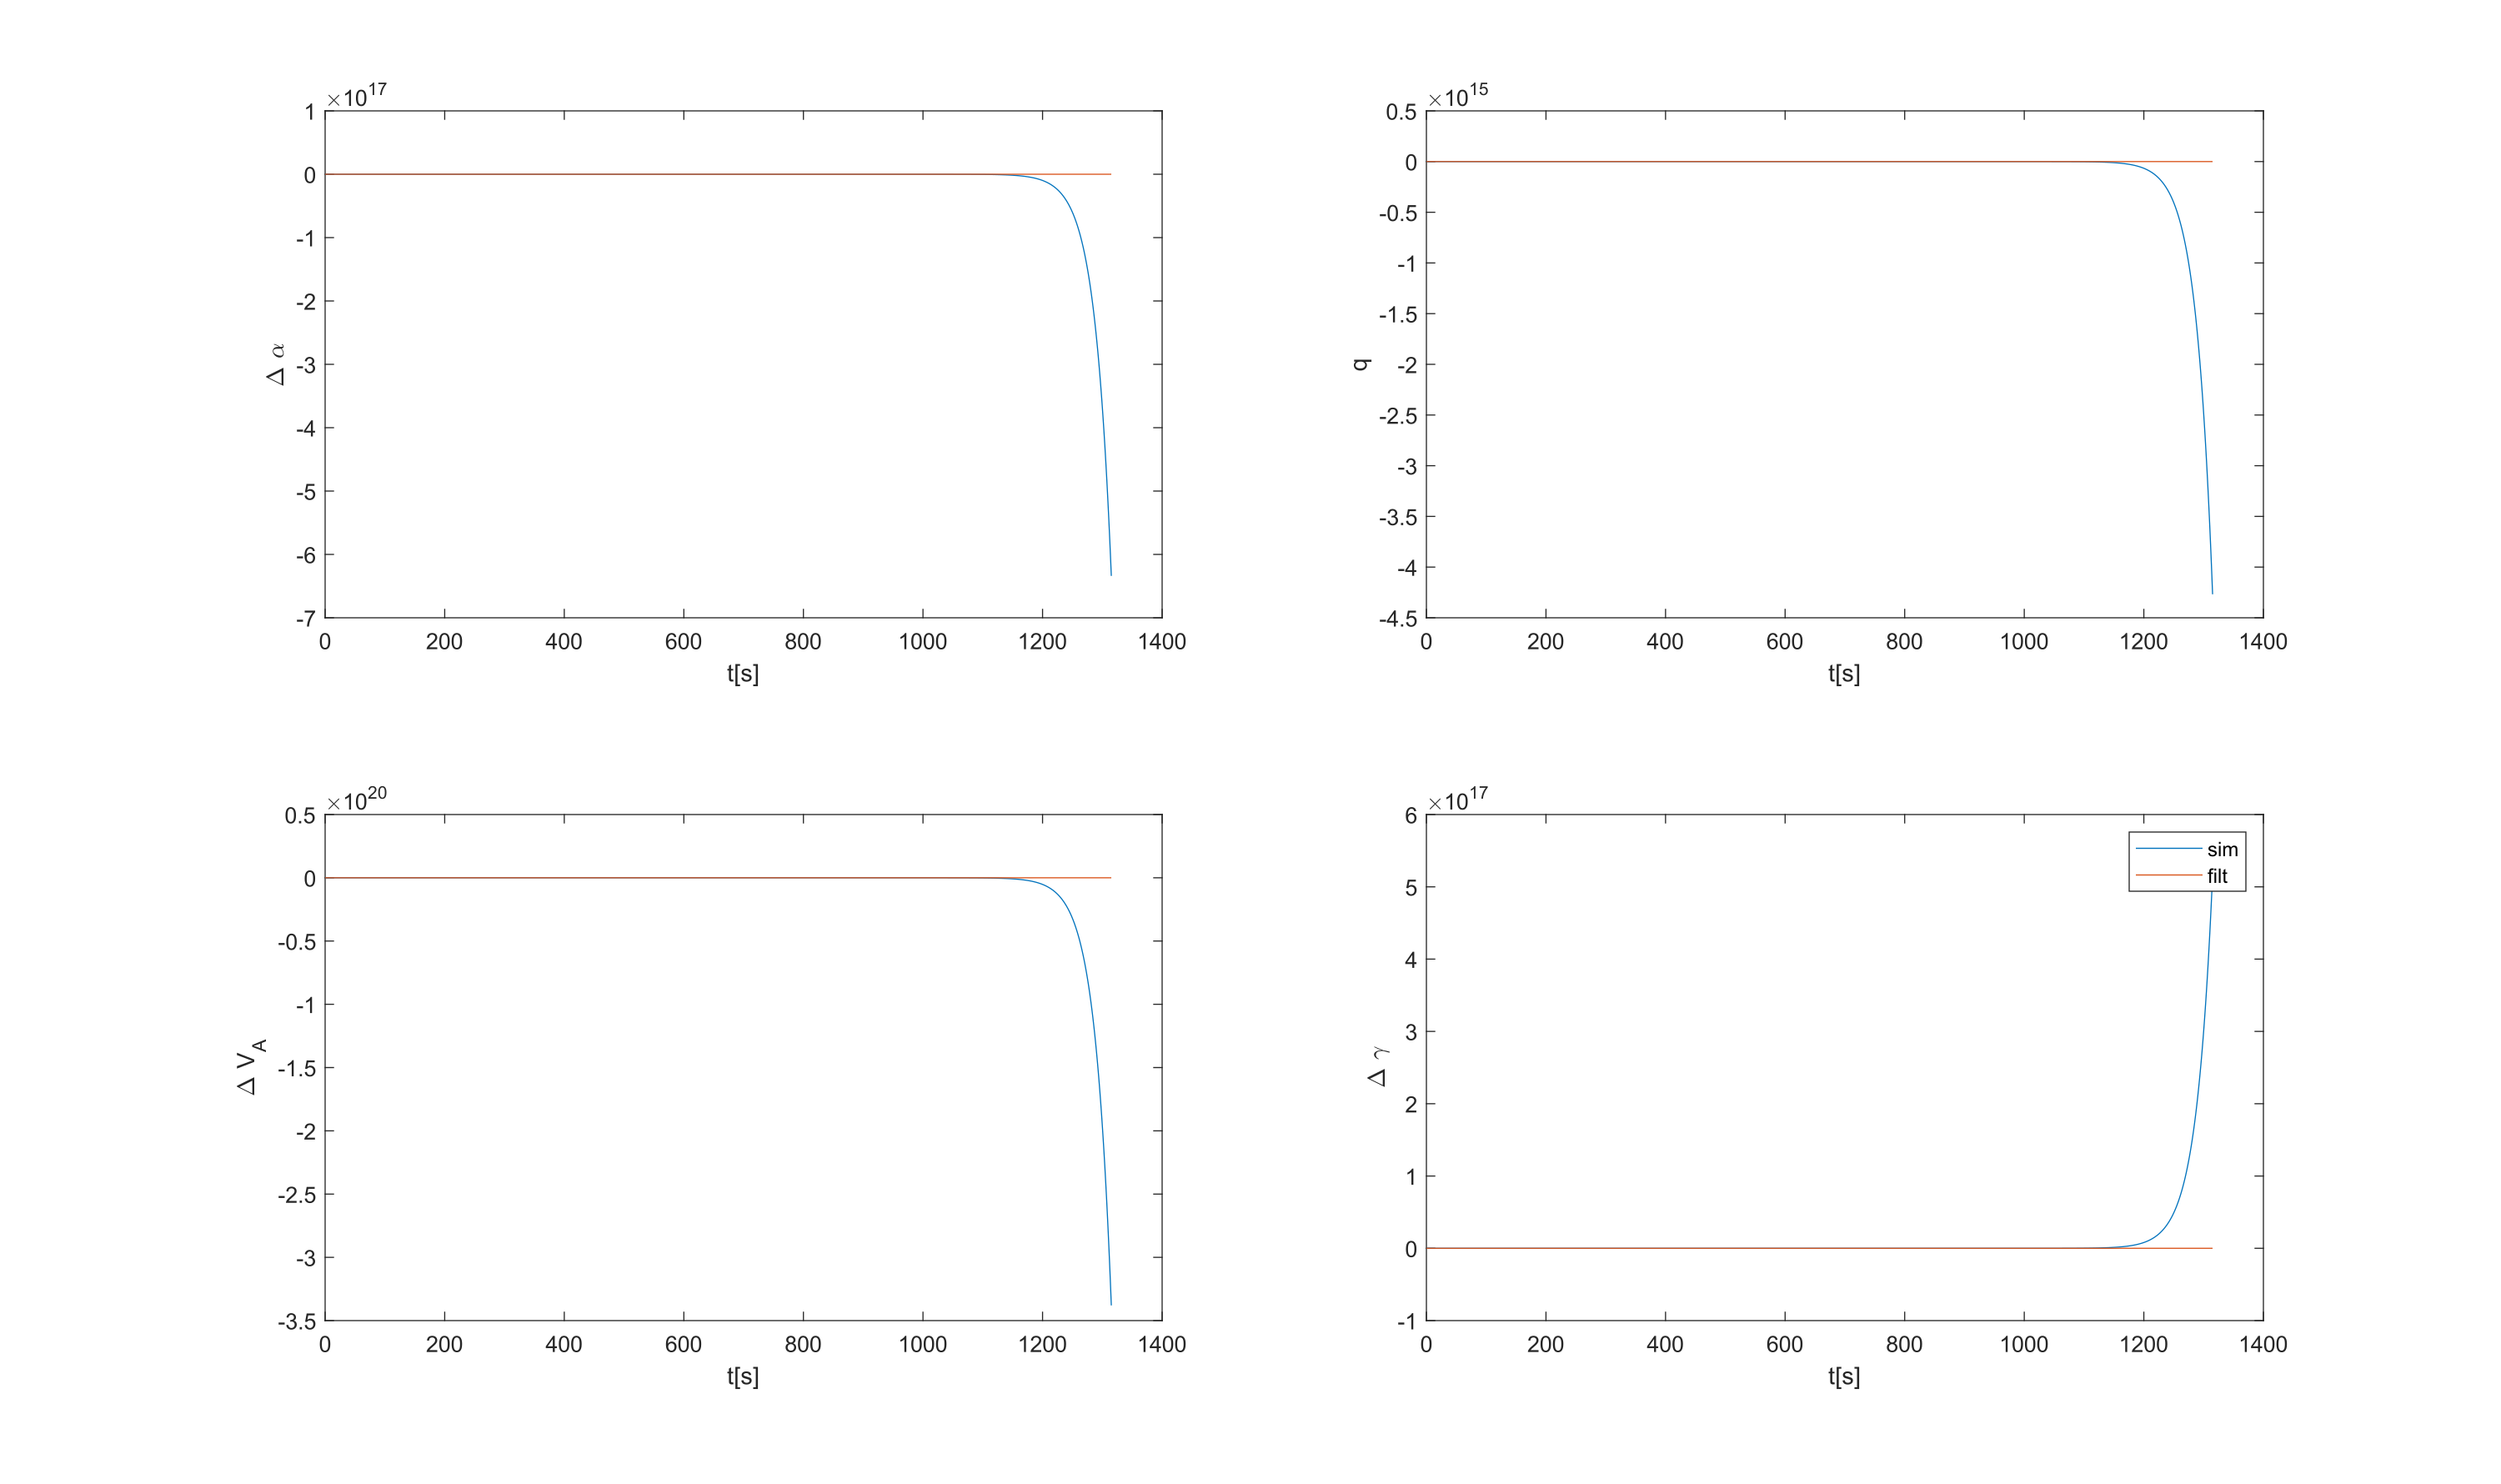
\includegraphics[trim=100 0 100 0,clip,width=1\linewidth]{LS_LSQ.png}
	\caption{Ergebnisse Anhand LSQ}
     \label{fig:Ergebnisse_zlsq} 
\end{figure}
